\def\sphoyear{2021}
\setcounter{section}{0}
% Headers and Descriptions
\fancyhead[L]{\textbf{SPhO \sphoyear}} \fancyhead[R]{\textbf{Questions}}


\begin{titlepage}
\centering

{\Huge\bfseries SPhO \sphoyear}

\vspace{1cm}

{\LARGE Problem Set}

\vspace{2cm}

{\Large Compiled by: Tan Chien Hao, \texttt{www.tchlabs.net}}

\vspace{2cm}

{\Large Edited/Proofread by: Keith Chan, Sun Yu Chieh}
%Collaborators please feel free to add on!

\vspace{2cm}

{\large Suggest changes at: \github}


\vfill

{\itshape Last edited: \today}
\end{titlepage}

\begin{problem}
    A parallel-plate capacitor is shown in the diagram with plate area of $A = \qty{10.5}{\cm}^2$ and plate separation $2d = \qty{7.12}{mm}$. The left half of the gap is filled with material of dielectric constant $\kappa_1 = 21.0$; the top of the right half is filled with material of dielectric constant $\kappa_2 = 42.0$; the bottom of the right half is filled with material of dielectric constant $\kappa_3 = 58.0$. What is the capacitance? \hfill $[4]$
    \begin{figure}[H]
        \centering
        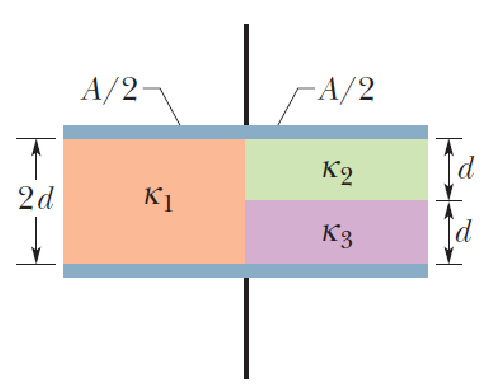
\includegraphics[width=0.5\textwidth]{spho_book_TYS_images/2021SPhO_1.png}
        \label{fig:1}
    \end{figure}
\end{problem}

\begin{problem}
    In the rectangle shown, the sides have lengths \qty{5.0}{\cm} and \qty{15}{\cm}, $q1 = \qty{-5.0}{\micro\C}$, and $q2 = \qty{+2.0}{\micro\C}$. 
    \begin{figure}[H]
        \centering
        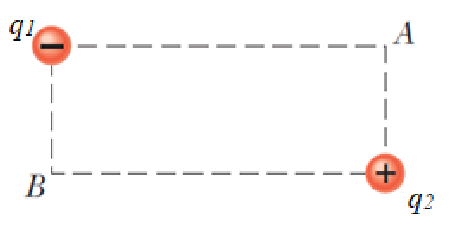
\includegraphics{spho_book_TYS_images/2021SPhO_2.png}
    \end{figure}  
    With  $V = 0$ at infinity, what is the electric potential at
    \begin{subproblemalph}
        \item corner A and \hfill $[1]$
        \item corner B? \hfill $[1]$
        \item How much work is required to move a charge $q3 = \qty{+3.0}{\micro\C}$ from B to A along a diagonal of the rectangle? \hfill $[1]$
        \item Does this work increase or decrease the electric potential energy of the three-charge system? \hfill $[1]$
    \end{subproblemalph}
    Is more, less, or the same work required if q3 is moved along a path that is
    \begin{subproblemalph}
        \setcounter{enumi}{4}
        \item inside the rectangle but not on a diagonal and \hfill $[0.5]$        
        \item outside the rectangle?  \hfill $[0.5]$
    \end{subproblemalph}
\end{problem}

\begin{problem}
    The conducting rod shown in the figure has length $L$ and is being pulled along horizontal, frictionless conducting rails at a constant velocity $\vec{v}$. The rails are connected at one end with a metal strip. A uniform magnetic field $\vec{B}$, directed out of the page, fills the region in which the rod moves. Assume that $L = 10 \unit{cm}$, $v = \qty{5.0}{\m\s^{-1}}$, and $B = \qty{1.2}{T}$. What are the
    \begin{subproblemalph}
        \item magnitude and \hfill [1]
        \item direction (up or down the page) of the emf induced in the rod? \hfill [0.5]
        \item magnitude and \hfill [0.5]
        \item direction of the current in the conducting loop? \hfill [0.5]
    \end{subproblemalph}
    Assume that the resistance of the rod is $0.40 \Omega$ and that the resistance of the rails and metal strip is negligibly small.
    \begin{subproblemalph}
        \setcounter{enumi}{4}
        \item At what rate is thermal energy being generated in the rod? \hfill [1]
        \item What external force on the rod is needed to maintain $\vec{v}$? \hfill [1.5]
        \item At what rate does this force do work on the rod? \hfill [1]
    \end{subproblemalph}
\end{problem}

\begin{problem}
    In the figure shown, after the switch S is closed at time $t = 0$, the emf of the source is automatically adjusted to maintain a constant current I through S.
    \begin{subproblemalph}
        \item Find the current through the inductor as
a function of time. \hfill [4]
        \item At what time is the current through the
resistor equal to the current through the
inductor? \hfill [1]
    \end{subproblemalph} 
\end{problem}